
%% bare_conf.tex
%% V1.4b
%% 2015/08/26
%% by Michael Shell
%% See:
%% http://www.michaelshell.org/
%% for current contact information.
%%
%% This is a skeleton file demonstrating the use of IEEEtran.cls
%% (requires IEEEtran.cls version 1.8b or later) with an IEEE
%% conference paper.
%%
%% Support sites:
%% http://www.michaelshell.org/tex/ieeetran/
%% http://www.ctan.org/pkg/ieeetran
%% and
%% http://www.ieee.org/

%%*************************************************************************
%% Legal Notice:
%% This code is offered as-is without any warranty either expressed or
%% implied; without even the implied warranty of MERCHANTABILITY or
%% FITNESS FOR A PARTICULAR PURPOSE!
%% User assumes all risk.
%% In no event shall the IEEE or any contributor to this code be liable for
%% any damages or losses, including, but not limited to, incidental,
%% consequential, or any other damages, resulting from the use or misuse
%% of any information contained here.
%%
%% All comments are the opinions of their respective authors and are not
%% necessarily endorsed by the IEEE.
%%
%% This work is distributed under the LaTeX Project Public License (LPPL)
%% ( http://www.latex-project.org/ ) version 1.3, and may be freely used,
%% distributed and modified. A copy of the LPPL, version 1.3, is included
%% in the base LaTeX documentation of all distributions of LaTeX released
%% 2003/12/01 or later.
%% Retain all contribution notices and credits.
%% ** Modified files should be clearly indicated as such, including  **
%% ** renaming them and changing author support contact information. **
%%*************************************************************************


% *** Authors should verify (and, if needed, correct) their LaTeX system  ***
% *** with the testflow diagnostic prior to trusting their LaTeX platform ***
% *** with production work. The IEEE's font choices and paper sizes can   ***
% *** trigger bugs that do not appear when using other class files.       ***                          ***
% The testflow support page is at:
% http://www.michaelshell.org/tex/testflow/



\documentclass[conference]{IEEEtran}
% Some Computer Society conferences also require the compsoc mode option,
% but others use the standard conference format.
%
% If IEEEtran.cls has not been installed into the LaTeX system files,
% manually specify the path to it like:
% \documentclass[conference]{../sty/IEEEtran}





% Some very useful LaTeX packages include:
% (uncomment the ones you want to load)


% *** MISC UTILITY PACKAGES ***
%
%\usepackage{ifpdf}
% Heiko Oberdiek's ifpdf.sty is very useful if you need conditional
% compilation based on whether the output is pdf or dvi.
% usage:
% \ifpdf
%   % pdf code
% \else
%   % dvi code
% \fi
% The latest version of ifpdf.sty can be obtained from:
% http://www.ctan.org/pkg/ifpdf
% Also, note that IEEEtran.cls V1.7 and later provides a builtin
% \ifCLASSINFOpdf conditional that works the same way.
% When switching from latex to pdflatex and vice-versa, the compiler may
% have to be run twice to clear warning/error messages.






% *** CITATION PACKAGES ***
%
%\usepackage{cite}
% cite.sty was written by Donald Arseneau
% V1.6 and later of IEEEtran pre-defines the format of the cite.sty package
% \cite{} output to follow that of the IEEE. Loading the cite package will
% result in citation numbers being automatically sorted and properly
% "compressed/ranged". e.g.,  without using
% cite.sty will become  using cite.sty. cite.sty's
% \cite will automatically add leading space, if needed. Use cite.sty's
% noadjust option (cite.sty V3.8 and later) if you want to turn this off
% such as if a citation ever needs to be enclosed in parenthesis.
% cite.sty is already installed on most LaTeX systems. Be sure and use
% version 5.0 (2009-03-20) and later if using hyperref.sty.
% The latest version can be obtained at:
% http://www.ctan.org/pkg/cite
% The documentation is contained in the cite.sty file itself.






% *** GRAPHICS RELATED PACKAGES ***
%
\ifCLASSINFOpdf
  \usepackage[pdftex]{graphicx}
  % declare the path(s) where your graphic files are
  % \graphicspath{{../pdf/}{../jpeg/}}
  % and their extensions so you won't have to specify these with
  % every instance of \includegraphics
  % \DeclareGraphicsExtensions{.pdf,.jpeg,.png}
\else
  % or other class option (dvipsone, dvipdf, if not using dvips). graphicx
  % will default to the driver specified in the system graphics.cfg if no
  % driver is specified.
  % \usepackage[dvips]{graphicx}
  % declare the path(s) where your graphic files are
  % \graphicspath{{../eps/}}
  % and their extensions so you won't have to specify these with
  % every instance of \includegraphics
  % \DeclareGraphicsExtensions{.eps}
\fi
% graphicx was written by David Carlisle and Sebastian Rahtz. It is
% required if you want graphics, photos, etc. graphicx.sty is already
% installed on most LaTeX systems. The latest version and documentation
% can be obtained at:
% http://www.ctan.org/pkg/graphicx
% Another good source of documentation is "Using Imported Graphics in
% LaTeX2e" by Keith Reckdahl which can be found at:
% http://www.ctan.org/pkg/epslatex
%
% latex, and pdflatex in dvi mode, support graphics in encapsulated
% postscript (.eps) format. pdflatex in pdf mode supports graphics
% in .pdf, .jpeg, .png and .mps (metapost) formats. Users should ensure
% that all non-photo figures use a vector format (.eps, .pdf, .mps) and
% not a bitmapped formats (.jpeg, .png). The IEEE frowns on bitmapped formats
% which can result in "jaggedy"/blurry rendering of lines and letters as
% well as large increases in file sizes.
%
% You can find documentation about the pdfTeX application at:
% http://www.tug.org/applications/pdftex





% *** MATH PACKAGES ***
%
%\usepackage{amsmath}
% A popular package from the American Mathematical Society that provides
% many useful and powerful commands for dealing with mathematics.
%
% Note that the amsmath package sets \interdisplaylinepenalty to 10000
% thus preventing page breaks from occurring within multiline equations. Use:
%\interdisplaylinepenalty=2500
% after loading amsmath to restore such page breaks as IEEEtran.cls normally
% does. amsmath.sty is already installed on most LaTeX systems. The latest
% version and documentation can be obtained at:
% http://www.ctan.org/pkg/amsmath





% *** SPECIALIZED LIST PACKAGES ***
%
%\usepackage{algorithmic}
% algorithmic.sty was written by Peter Williams and Rogerio Brito.
% This package provides an algorithmic environment fo describing algorithms.
% You can use the algorithmic environment in-text or within a figure
% environment to provide for a floating algorithm. Do NOT use the algorithm
% floating environment provided by algorithm.sty (by the same authors) or
% algorithm2e.sty (by Christophe Fiorio) as the IEEE does not use dedicated
% algorithm float types and packages that provide these will not provide
% correct IEEE style captions. The latest version and documentation of
% algorithmic.sty can be obtained at:
% http://www.ctan.org/pkg/algorithms
% Also of interest may be the (relatively newer and more customizable)
% algorithmicx.sty package by Szasz Janos:
% http://www.ctan.org/pkg/algorithmicx




% *** ALIGNMENT PACKAGES ***
%
%\usepackage{array}
% Frank Mittelbach's and David Carlisle's array.sty patches and improves
% the standard LaTeX2e array and tabular environments to provide better
% appearance and additional user controls. As the default LaTeX2e table
% generation code is lacking to the point of almost being broken with
% respect to the quality of the end results, all users are strongly
% advised to use an enhanced (at the very least that provided by array.sty)
% set of table tools. array.sty is already installed on most systems. The
% latest version and documentation can be obtained at:
% http://www.ctan.org/pkg/array


% IEEEtran contains the IEEEeqnarray family of commands that can be used to
% generate multiline equations as well as matrices, tables, etc., of high
% quality.

\usepackage{amsmath}
\usepackage{enumitem}
\usepackage{caption}% http://ctan.org/pkg/caption
\captionsetup[table]{format=plain,labelformat=simple,labelsep=period}%
\captionsetup{skip=0pt}

\renewcommand\IEEEkeywordsname{Index Terms}


% *** SUBFIGURE PACKAGES ***
%\ifCLASSOPTIONcompsoc
%  \usepackage[caption=false,font=normalsize,labelfont=sf,textfont=sf]{subfig}
%\else
%  \usepackage[caption=false,font=footnotesize]{subfig}
%\fi
% subfig.sty, written by Steven Douglas Cochran, is the modern replacement
% for subfigure.sty, the latter of which is no longer maintained and is
% incompatible with some LaTeX packages including fixltx2e. However,
% subfig.sty requires and automatically loads Axel Sommerfeldt's caption.sty
% which will override IEEEtran.cls' handling of captions and this will result
% in non-IEEE style figure/table captions. To prevent this problem, be sure
% and invoke subfig.sty's "caption=false" package option (available since
% subfig.sty version 1.3, 2005/06/28) as this is will preserve IEEEtran.cls
% handling of captions.
% Note that the Computer Society format requires a larger sans serif font
% than the serif footnote size font used in traditional IEEE formatting
% and thus the need to invoke different subfig.sty package options depending
% on whether compsoc mode has been enabled.
%
% The latest version and documentation of subfig.sty can be obtained at:
% http://www.ctan.org/pkg/subfig




% *** FLOAT PACKAGES ***
%
%\usepackage{fixltx2e}
% fixltx2e, the successor to the earlier fix2col.sty, was written by
% Frank Mittelbach and David Carlisle. This package corrects a few problems
% in the LaTeX2e kernel, the most notable of which is that in current
% LaTeX2e releases, the ordering of single and double column floats is not
% guaranteed to be preserved. Thus, an unpatched LaTeX2e can allow a
% single column figure to be placed prior to an earlier double column
% figure.
% Be aware that LaTeX2e kernels dated 2015 and later have fixltx2e.sty's
% corrections already built into the system in which case a warning will
% be issued if an attempt is made to load fixltx2e.sty as it is no longer
% needed.
% The latest version and documentation can be found at:
% http://www.ctan.org/pkg/fixltx2e


%\usepackage{stfloats}
% stfloats.sty was written by Sigitas Tolusis. This package gives LaTeX2e
% the ability to do double column floats at the bottom of the page as well
% as the top. (e.g., "\begin{figure*}[!b]" is not normally possible in
% LaTeX2e). It also provides a command:
%\fnbelowfloat
% to enable the placement of footnotes below bottom floats (the standard
% LaTeX2e kernel puts them above bottom floats). This is an invasive package
% which rewrites many portions of the LaTeX2e float routines. It may not work
% with other packages that modify the LaTeX2e float routines. The latest
% version and documentation can be obtained at:
% http://www.ctan.org/pkg/stfloats
% Do not use the stfloats baselinefloat ability as the IEEE does not allow
% \baselineskip to stretch. Authors submitting work to the IEEE should note
% that the IEEE rarely uses double column equations and that authors should try
% to avoid such use. Do not be tempted to use the cuted.sty or midfloat.sty
% packages (also by Sigitas Tolusis) as the IEEE does not format its papers in
% such ways.
% Do not attempt to use stfloats with fixltx2e as they are incompatible.
% Instead, use Morten Hogholm'a dblfloatfix which combines the features
% of both fixltx2e and stfloats:
%
% \usepackage{dblfloatfix}
% The latest version can be found at:
% http://www.ctan.org/pkg/dblfloatfix




% *** PDF, URL AND HYPERLINK PACKAGES ***
%
%\usepackage{url}
% url.sty was written by Donald Arseneau. It provides better support for
% handling and breaking URLs. url.sty is already installed on most LaTeX
% systems. The latest version and documentation can be obtained at:
% http://www.ctan.org/pkg/url
% Basically, \url{my_url_here}.




% *** Do not adjust lengths that control margins, column widths, etc. ***
% *** Do not use packages that alter fonts (such as pslatex).         ***
% There should be no need to do such things with IEEEtran.cls V1.6 and later.
% (Unless specifically asked to do so by the journal or conference you plan
% to submit to, of course. )


% correct bad hyphenation here
\hyphenation{op-tical net-works semi-conduc-tor}


\begin{document}
%
% paper title
% Titles are generally capitalized except for words such as a, an, and, as,
% at, but, by, for, in, nor, of, on, or, the, to and up, which are usually
% not capitalized unless they are the first or last word of the title.
% Linebreaks \\ can be used within to get better formatting as desired.
% Do not put math or special symbols in the title.
\title{A Three-Layer Hybrid Model for Wind Power Prediction}


% author names and affiliations
% use a multiple column layout for up to three different
% affiliations
\author{\IEEEauthorblockN{Jian Gao}
\IEEEauthorblockA{Computer Science \& Engineering Department \\
New York University, New York, NY 10003 \\
Email: jg4631@nyu.edu}
\and
\IEEEauthorblockN{Panitarn Chongfuangprinya, Yanzhu Ye, Bo Yang}
\IEEEauthorblockA{Energy Solution Laboratory, R\&D \\ Hitachi America Ltd, Santa Clara, CA 95054 \\
Email: \{joseph.chong, yanzhu.ye, bo.yang\}@hal.hitachi.com}
% \and
% \IEEEauthorblockN{TBD}
% \IEEEauthorblockA{Big Data Laboratory, R\&D Division \\ Hitachi America, Ltd \\
% Santa Clara, California, 95054\\
% Telephone: (000) 000--0000\\
% Fax: (000) 000--0000}
}

% conference papers do not typically use \thanks and this command
% is locked out in conference mode. If really needed, such as for
% the acknowledgment of grants, issue a \IEEEoverridecommandlockouts
% after \documentclass

% for over three affiliations, or if they all won't fit within the width
% of the page, use this alternative format:
%
%\author{\IEEEauthorblockN{Michael Shell\IEEEauthorrefmark{1},
%Homer Simpson\IEEEauthorrefmark{2},
%James Kirk\IEEEauthorrefmark{3},
%Montgomery Scott\IEEEauthorrefmark{3} and
%Eldon Tyrell\IEEEauthorrefmark{4}}
%\IEEEauthorblockA{\IEEEauthorrefmark{1}School of Electrical and Computer Engineering\\
%Georgia Institute of Technology,
%Atlanta, Georgia 30332--0250\\ Email: see http://www.michaelshell.org/contact.html}
%\IEEEauthorblockA{\IEEEauthorrefmark{2}Twentieth Century Fox, Springfield, USA\\
%Email: homer@thesimpsons.com}
%\IEEEauthorblockA{\IEEEauthorrefmark{3}Starfleet Academy, San Francisco, California 96678-2391\\
%Telephone: (800) 555--1212, Fax: (888) 555--1212}
%\IEEEauthorblockA{\IEEEauthorrefmark{4}Tyrell Inc., 123 Replicant Street, Los Angeles, California 90210--4321}}




% use for special paper notices
%\IEEEspecialpapernotice{(Invited Paper)}




% make the title area
\maketitle

% As a general rule, do not put math, special symbols or citations
% in the abstract
\begin{abstract}
Accurate wind power prediction (WPP) is important for stable operation of power systems. However, the intermittent nature and high variability of wind causes many challenges. This paper proposes a three-layer WPP model considering the data from historical power measurements and numerical weather prediction (NWP) systems. The first layer uses a linear model to learn the wind power generation equation. The second layer includes several non-linear models to learn the seasonality and the inertia of wind turbines. The third layer uses stacked regression to learn a hybrid combination of predictors in the previous layer. We compared the proposed approach against the state-of-the-art algorithm as well as two neural network models. Experiment results show that our approach has the best performance.

%Renewable energy such as wind, solar and hydropower has a rapid growth in the past decades. These energy resources give utility companies the opportunity to provide clean and economical services, which benefits both the customers and our environment. However, the intermittent nature and high variability of wind power generation causes many challenges to power system operators. An accurate wind power prediction system is very essential for economic and stable operation of the electricity markets. In this work, the problem of wind power prediction (WPP) is addressed. We proposed a three-layer WPP model considering the data from historical power measurements and numerical weather prediction (NWP) systems. The first layer is a linear model that learns the wind power generation equation of wind turbines. The second layer consists of several non-linear models that learn the seasonality and the inertia of wind turbines. The third layer is a stacked regression model that forms linear combinations of the predictors from the previous layer. We compared the proposed approach against the state-of-the-art algorithm as well as several neural network models. Experiment results show our approach has the best performance.

% Distributed energy  resources (DER) such as solar farms, rooftop PV systems etc have grown to be a major asset in US electricity market due to their clean form of energy. California state is committed to provide 50\% of its consumer electricity demand through the DERs by 2030. However, high penetration of these DERs in the power grid results in bad quality of electricity that leads to voltage fluctuations and sometimes even a system level blackout due to tripping of protection system, etc. In this work, a new modelling framework is proposed that enables the utilities/solar farm investors to calculate the maximum capacity of solar farm that can be integrated into the system without any undesirable behavior in the power grid. Currently, the utilities do not yet have a solid solution for this problem and they have been working on it for several years. Within the case study, a node-by-node integration capacity analysis (ICA) is carried out to obtain the ICA values using an iterative algorithm. It turns out that this integration capacity value is highly location dependent and can be further affected by network topology. A binary search technique is used to reduce the computational complexity of the algorithm. New visualization tools were developed to collect the graphical information of power grid from a code based file and it also provides various heat maps, system parameter monitoring, etc. This work enables the utilities to give permits to the solar farm investors to install solar farms at viable locations. The future scope of this work includes using reinforcement learning and data analytics to reduce the computation time of the iterative algorithm and also to solve a more improvised version of ICA problem. This creates a smart AI system to support the power system control operator in the control room.






%These resources enable utility companies to provide cheaper and cleaner energy services.

%The stability and operation of electric power system is mainly governed by demand and supply balance.


%has led to a significant growth in renewable energy conversion systems in the last few decades.

%is rapidly increasing as alternatives


\end{abstract}

\begin{IEEEkeywords}
wind power, time series, hybrid model, long-term forecasting, renewable energy.
\end{IEEEkeywords}




% For peer review papers, you can put extra information on the cover
% page as needed:
% \ifCLASSOPTIONpeerreview
% \begin{center} \bfseries EDICS Category: 3-BBND \end{center}
% \fi
%
% For peerreview papers, this IEEEtran command inserts a page break and
% creates the second title. It will be ignored for other modes.
\IEEEpeerreviewmaketitle



\section{Introduction}
% no \IEEEPARstart
Under the pressure of global warming and environment pollution, renewable energy systems have a rapid growth in the past decades. %Renewable energy resources such as wind farms, solar energy have grown to be a major asset in US electricity market due to their clean form of energy. Many countries have launched projects for large-scale integration of renewable energy resources into their grids. The state of California is committed to provide 50\% of its consumer electricity demand through the renewable energy by 2030.
The increasing integration of wind and solar power generation leads to potential impacts on planning and operations of power systems. Utilities need to maintain the balance of demand and supply to ensure the stability of electric power operation. However, the intermittent nature and high variability of wind power generation causes many challenges to power system operators. %Recent adaptations to national grid codes require wind farms to contribute to voltage regulation in the system as the conventional power plants do \cite{8778495}. They must have the ability to generate or absorb reactive power in order to influence the voltage level at the point of common coupling (PCC) \cite{MOHSENI20123876}. Energy forecasting can help to integrate wind power generation into conventional power system and satisfy the grid code.
A robust and accurate wind power prediction (WPP) system is very essential for economic and stable operation of the electricity markets.

According to several studies in this area \cite{LAZIC2014567,8489472}, WPP approaches can be classified based on the forecasting horizon into three categories \cite{WANG2011770}:
\begin{itemize}
\item Short-term forecasting (minutes to 8 hours-ahead)
\item Mid-term forecasting (8 hours to day-ahead)
\item Long-term forecasting (multiple-days-ahead)
\end{itemize}
A long-term wind power forecasting system gives utilities time to maintain system frequency and operating reserve, which benefits bidding in multiple-days-ahead electricity markets.

Wind power forecasting can be classified into physical approaches, statistical approaches, and hybrid approaches \cite{LI201356,Gao2016DistributedMF,Alencar17}. Physical approaches take into account the physical characteristic of the wind power generation process and establish a mathematical model from wind force to electric energy production, where accurate wind strength measurement is required. These approaches are effective in short-term forecasting and useful in dealing with operation problems. Statistical approaches learn the underlying non-linear relation between numerical weather prediction (NWP) wind forecasting and wind power generation through statistical methods. In general, NWP forecasts have major impact on the WPP performance.

Pierre Huyn et al. \cite{Pierre17} developed a machine learning model based on support vector machines (SVMs) to forecast day-ahead wind power generation in 15-minute intervals. Shu Fan et al. \cite{4757294} designed a model using Bayesian clustering and SVM to learn the NWP wind speed forecasting patterns. Bhaskar Kanna and Sri Niwas Singh \cite{7894735} proposed an adaptive wavelet neural network (AWNN) to learn the mapping from NWP’s wind speed and wind direction forecasts to wind power forecasts. Yao Liu et al. \cite{app9061108} provided a short-term wind forecasting model based on discrete wavelet transform and long short-term memory networks (DWT\_LSTM). However, due to the large time scale in long-term forecasting and the noisy outputs of weather forecasting systems, short-term methods cannot be directly used. The industry has not established effective approaches for long-term forecasting \cite{HAN2019181}.

This work addresses the problem of long-term wind power prediction. We proposed a three-layer WPP model considering the data from historical power measurements and NWP systems. The first layer learns the physical relation between wind force and wind power generation by modeling the wind generation process of wind turbines. It maps NWP’s wind speed and wind direction forecasts to a basic wind power estimation based on a linear model. The second layer consists of several non-linear models that learn the seasonality and the inertia of wind turbines. The third layer is a stacked regression model that forms linear combinations of the predictors from the previous layer. The proposed approach is tested on a public dataset, in which the task is to predict 48-hour ahead hourly wind power generation at 7 wind farms. The prediction accuracy is evaluated by Root Mean Square Error (RMSE) and Mean Absolute Error (MAE). We compared the proposed approach against the state-of-the-art algorithm as well as several neural network models. Experiment results show our approach has the best performance.

This paper is organized as follows: Section II introduces the problem and a brief description of the dataset. Section III provides detailed explanation of the proposed algorithms. Section IV shows the performance evaluation and comparison. Section V concludes the paper.

% You must have at least 2 lines in the paragraph with the drop letter
% (should never be an issue)
%I wish you the best of success.

%\hfill mds

%\hfill August 23, 2019



\section{Problem Description}

\subsection{The Problem}
We study the problem of WPP. The task is to predict 48-hour ahead hourly wind power generation at 7 wind farms. Available information in the training data contains historical power measurements of these wind farms and meteorological forecasts of wind components from the NWP systems at each farm. The actual wind power generation was measured and recorded hourly and denoted by $wp[t]$. The NWP meteorological forecasts are formulated as vectors containing the predicted wind speed and wind direction ($ws_k, wd_k$), $k=1,...,K$, where $K$ is the total number of forecasting records. The NWP forecasts were issued twice a day at time $t_k$ with forecasting horizon of 48 hours ahead.
\begin{equation}
\begin{aligned}
ws_k &= \{ ws[t] \mid t = t_k + 1,..., t_k + 48 \} \\
wd_k &= \{ wd[t] \mid t = t_k + 1,..., t_k + 48 \}
\end{aligned}
\end{equation}
Similarly, the wind power generation is predicted in hourly resolution. The WPP model will learn the mapping from the current NWP wind forecasts and the actual wind power measurement in the past. It can be described by
\begin{equation}
\hat{wp}[t] = f(ws[t], wd[t], wp[t-i], \Theta) \quad i = 1, 2, ...
\end{equation}
where $\Theta$ denotes the model parameters learnt from the existing observations. When new NWP forecasts come, the model forecasts the wind power generation at the corresponding hour. %Figure \ref{fig:architecture} shows the high-level architecture of WPP.
%\begin{figure}
%\centering
%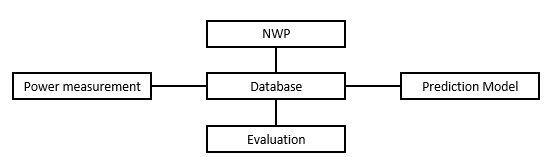
\includegraphics[width=0.9\columnwidth]{FIG/architecture.jpg}
%\caption{High-level Architecture of WPP}
%\label{fig:architecture}
%\end{figure}


A major challenge of this problems comes from the unpredictable nature and variability of wind conditions, especially the difference between meteorological wind forecasts and the actual wind condition at specific wind farm locations and altitudes due to microclimate. Another issue is the time-series nature of the data that inherits the long-term dependencies and seasonal effects of wind. Traditional time-series models like Autoregressive Integrated Moving Average (ARIMA) cannot formulate such non-linear relationships and incorporate all these effects. We address those issues by training a hybrid model and extract features from the following three aspects:
\begin{enumerate}
\item Meteorological wind forecasts from NWP
\item Environmental influence of season and farm location
%  \begin{enumerate}
%    \item Season impact
%    \item Location impact
%  \end{enumerate}
\item Historical data of past wind power measurement
%  \begin{enumerate}
%    \item The entire historical value (to capture the trend)
%    \item The most recent wind power generation (to capture the inertia of windmills)
%  \end{enumerate}
\end{enumerate}

For long-term wind power prediction ($> 24$ hours), features from aspect 1) and 2) show more contribution to the prediction performance. The prediction is made by solving a supervised learning problem, and no specific time-series model was used. Therefore, we need to design handcraft features for historical data to capture the time-series property in data streams.


\subsection{The Data}
The data is collected from Global Energy Forecasting Competition 2012 - Wind Forecasting \cite{HONG2014357}. It consists of NWP wind speed \& direction forecasts and actual wind power measurement. %All power values are normalized between 0 and 1 to hide the original characteristics of the wind farms, such as the location and actual weather information.
All power values have hourly resolution and were normalized between 0 and 1. This enables a scale-free comparison of the forecasting results on various wind farms. The NWP forecast outputs are available twice daily at 00UTC and 12UTC and has forecast horizon of 48 hours ahead. Thus, for each datetime, there are 4 NWP forecasts with different forecast horizons. Figure \ref{fig:pattern} shows the NWP forecast pattern.
%\begin{table}
%\caption {Missing Patterns in the First Period}
%\begin{center}
%\resizebox{\columnwidth}{!}{
%\begin{tabular}{|c|c|c|c|c|c|c|c|}
%\hline
%pos             & 1-12 & 13-24 & 25-36 & 37-48 & 49-60 & 61-72 & 73-84 \\ \hline
%horizon         & N/A  & N/A   & N/A   & 1-12  & 13-24 & 25-36 & 37-48 \\ \hline
%\textit{wp}     & 1    & 1     & 1     & 1     & 1     & 1     & 1     \\ \hline
%NWP             & 4    & 4     & 4     & 4     & 4     & 4     & 4     \\ \hline
%\end{tabular}
%}
%\label{tab:first}
%\end{center}
%\vspace*{-5mm}
%\end{table}

\begin{figure}
\centering
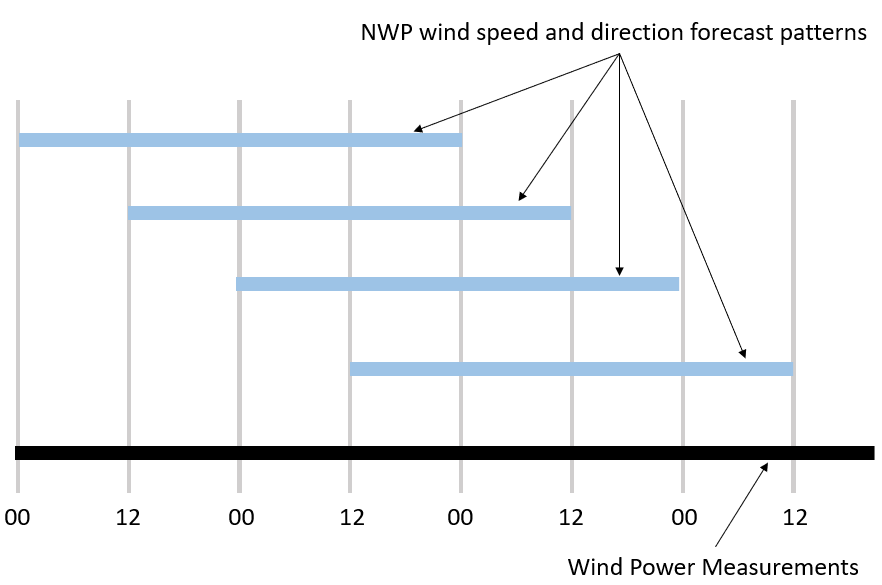
\includegraphics[width=0.7\columnwidth]{FIG/pattern}
\caption{NWP Forecast Patterns}
\label{fig:pattern}
\vspace*{-5mm}
\end{figure}

There are two parts of available data (yyyy-mm-dd-hh):
\begin{itemize}
\item Series for the period 2009-07-01-00 to 2010-12-30-12
\item Series for the period 2010-12-30-13 to 2012-06-28-12
\end{itemize}
In the first part, both actual power and wind forecasting are available at all datetimes. In the second part, a set of 48-hour periods with missing power observations are left for prediction. Each part can be split into 156 ``$84-hour$ blocks".
%The first one is from 2011-01-01-01 to 2011-01-03-00, followed by 36-hour available period. The second one is from 2011-01-04-13 to 2011-01-06-12, followed by the second 36-hour available data. The last one is from 2012-06-26-13 to 2012-06-28-12, without data followed. Figure \ref{fig:missing} shows the missing pattern in the second period. Both parts can be split into 156 batches, with 84 hours in each. Note that, in the second period, only the meteorological forecasts that were relevant for the periods with missing power data, which would be available in practice, were given \cite{HONG2014357}. Thus,
%In the second part, the number of NWP forecasts at each hour various from 1 to 4. The missing pattern depends on prediction horizons, as shown in Table \ref{tab:second}. %of wind power and NWP forecasts in the second period.

%\begin{table}
%\caption {Missing Patterns in the Second Period}
%\begin{center}
%\resizebox{\columnwidth}{!}{
%\begin{tabular}{|c|c|c|c|c|c|c|c|}
%\hline
%pos             & 1-12 & 13-24 & 25-36 & 37-48 & 49-60 & 61-72 & 73-84 \\ \hline
%horizon         & N/A  & N/A   & N/A   & 1-12  & 13-24 & 25-36 & 37-48 \\ \hline
%\textit{wp}     & 1    & 1     & 1     & 0     & 0     & 0     & 0     \\ \hline
%NWP             & 4    & 4     & 4     & 4     & 3     & 2     & 1     \\ \hline
%\end{tabular}
%}
%\label{tab:second}
%\end{center}
%\vspace*{-5mm}
%\end{table}

%\begin{figure}
%\centering
%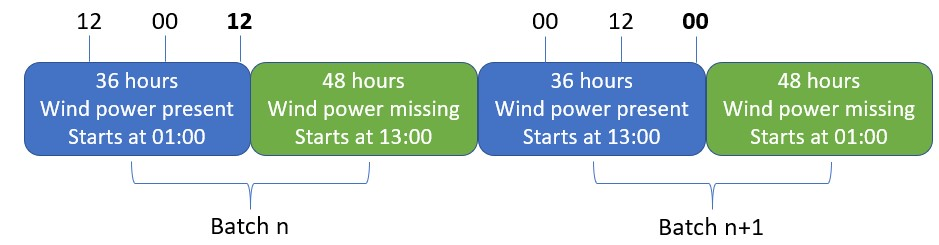
\includegraphics[width=0.9\columnwidth]{FIG/missing}
%\caption{NWP Forecast Patterns}
%\label{fig:missing}
%\end{figure}


%\subsection{Data Analysis}
%Figure \ref{fig:hist} shows the probability distribution histogram of wind speed and wind direction of all available data. The mean and maximum wind speed is around 4.6 and 17.0 m/s. Since the wind blow is not uniform in all directions, we can include wind direction as a feature.
%\begin{figure}
%\centering
%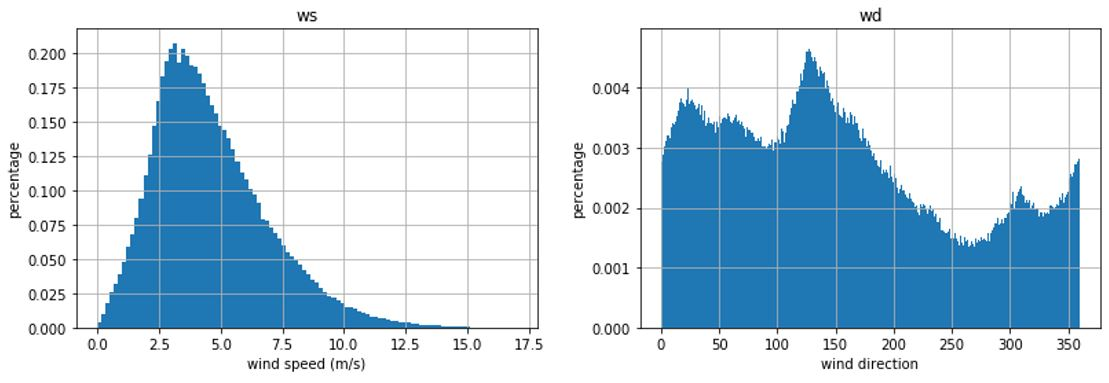
\includegraphics[width=0.9\columnwidth]{FIG/hist}
%\caption{Distribution of wind speed and wind direction}
%\label{fig:hist}
%\end{figure}
%
%Figure \ref{fig:pearson} left shows the correlation between wind speed and wind power generation. It demonstrates strong linear relationship, so we can use linear model to learn the wind power generation equation. The correlation between wind direction and wind power generation is displayed in Figure \ref{fig:pearson} right, which shows strong non-linear relationship. This suggests using categorical variable to represent wind direction.
%\begin{figure}
%\centering
%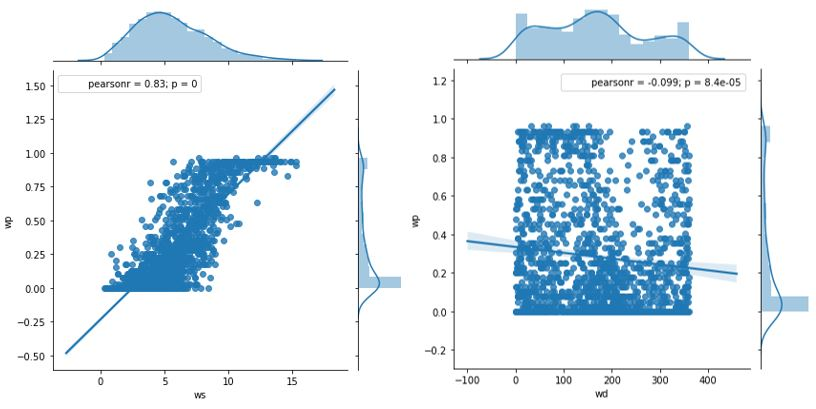
\includegraphics[width=0.9\columnwidth]{FIG/pearson}
%\caption{The correlation with wind power}
%\label{fig:pearson}
%\end{figure}
%
%Figure \ref{fig:season} illustrates the monthly and hourly seasonality of wind power generation. It shows obvious monthly seasonal pattern, so that we can extract month as an important feature. Hourly wind power is almost uniform throughout the day. Therefore, we do not include this type of feature. Another finding is that, the wind power has lowest value in July 15 and shows symmetric pattern. So, we create a feature by counting the days away from July 15: $|x-195|$, where x is the day in a year, and 195 is the day of July 15 in a year.
%\begin{figure}
%\centering
%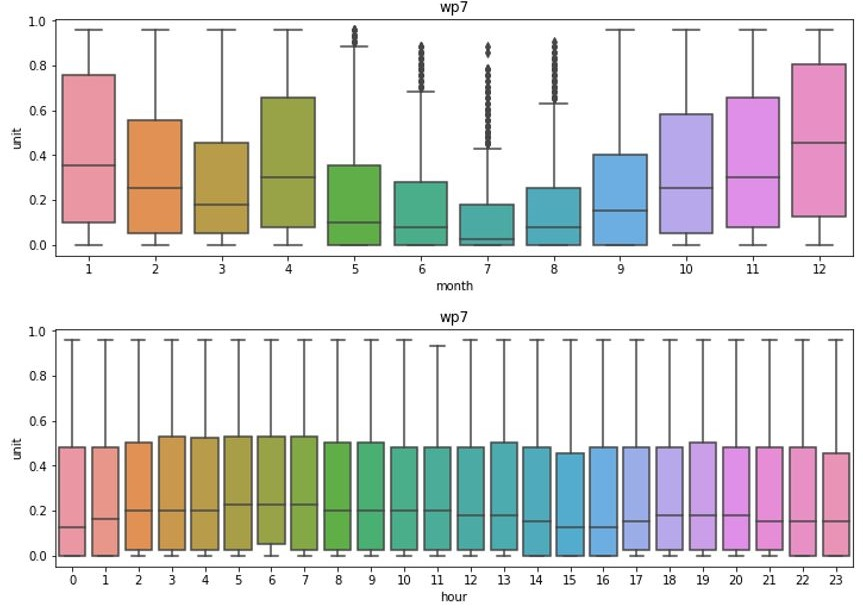
\includegraphics[width=0.9\columnwidth]{FIG/season}
%\caption{Seasonality in month (top) and hour (bottom)}
%\label{fig:season}
%\end{figure}
%
%To analysis the lag correlation of time-series data, we plot the auto-correlation of wind power generation in Figure \ref{fig:auto}. It shows strong auto-correlation between T-1, T, and T+1.
%\begin{figure}
%\centering
%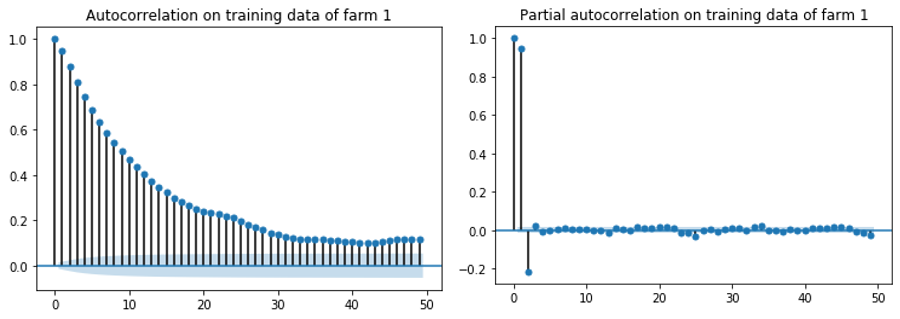
\includegraphics[width=0.9\columnwidth]{FIG/auto}
%\caption{Auto-correlation of Wind Power Generation}
%\label{fig:auto}
%\end{figure}
%
%Although the farms’ locations are not released, we can still get some hint from the dataset. Figure \ref{fig:farm} shows the correlation of the wind power generation on each farm pair. We found strong relationship between farm 4, farm 6 and farm 7. This information is useful for designing prediction models. \begin{figure}
%\centering
%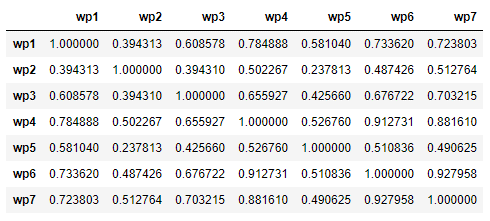
\includegraphics[width=0.9\columnwidth]{FIG/farm}
%\caption{Wind Power Correlation between Farms}
%\label{fig:farm}
%\end{figure}
%


\section{Proposed Method}
%Wind power generation is a non-linear and non-stationary time series \cite{WANG2017977}, which is very difficult to forecast due to the intermittent and unstable nature of wind. Since the ability of single model is limited, people use hybrid models to integrate information. The most common combinations are physical and statistical models, short-term and long-term models, and alternative machine learning models \cite{Chang14}.

We propose a three-layer hybrid model to predict the wind power generation, in which each layer takes the output of previous layer as input data, and produce its own predictions. %The first layer is a linear model that learns the wind power generation equation of wind turbines. It maps NWP wind speed and wind direction forecasts to a basic wind power estimation. The second layer consists of several non-linear models that learn the seasonality and the inertia of wind turbines. The third layer is a stacked regression model that forms a linear combination of the predictors in the previous layer.
Figure \ref{fig:flowchart} describes the entire system. %main functional components of the proposed WPP system. The detailed components of these models are explained in the following subsections.
\begin{figure}[b]
\centering
\vspace*{-5mm}
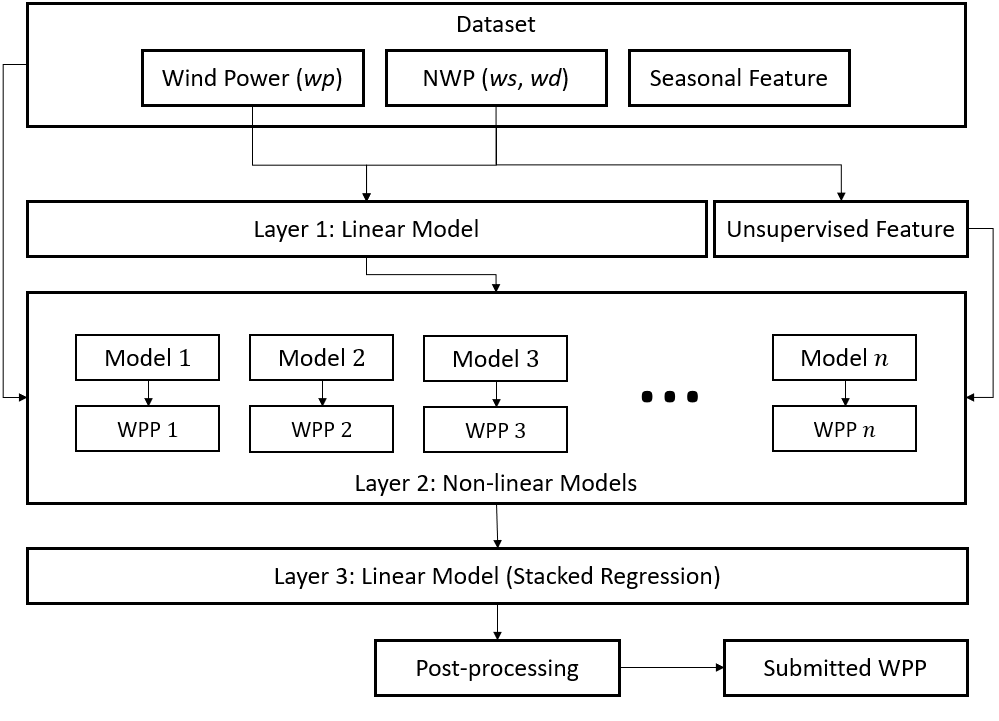
\includegraphics[width=0.9\columnwidth]{FIG/flowchart}
\caption{The Three Layer Wind Power Prediction Framework}
\label{fig:flowchart}
\end{figure}

\subsection{First Layer Prediction}
Accurate NWP wind forecasting is decisive to train a good WPP system \cite{WANG20171345}. The first layer model uses NWP data to learn the wind power generation equation of wind turbines.

Wind power is generated from the impact between wind and the blades of wind turbines. The rotating blades slow down the wind and convert it to mechanical energy that drives rotor to generate electricity. %The proportion of wind power that can be extracted by wind turbine is described in Figure \ref{fig:turbine}, where the conversion rate $C_p$ is limited to $59\%$ by Betz$'$s Law.
\begin{figure}[htb]
\centering
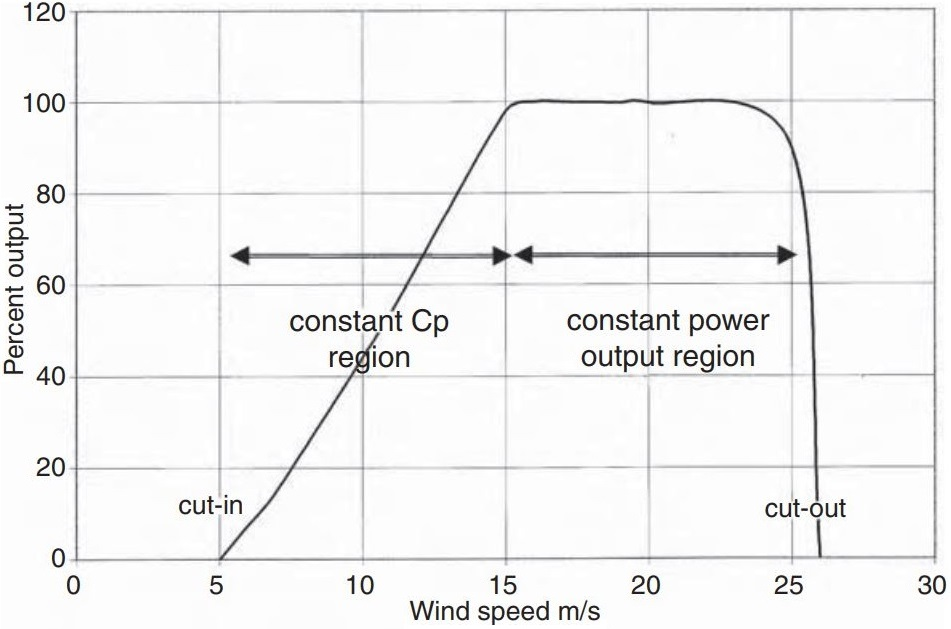
\includegraphics[width=0.7\columnwidth]{FIG/turbine}
\caption{Three Regions of Turbine speed Control \cite{patel2005wind}}
\label{fig:turbine}
\vspace*{-5mm}
\end{figure}
The speed-power curve can be split into three regions (Figure \ref{fig:turbine}) according to the convergence rate $C_p$:
\begin{enumerate}
    \item Constant $C_p$ region, power linearly increases with wind
    \item Constant power region, power reaches a controlled limit
    \item Region of power shutdown, wind exceeds the upper limit
\end{enumerate}
The electric energy comes from the kinetic energy of wind, which is a function of the wind speed ($ws$) and air mass ($m$). The kinetic energy of wind is
\begin{equation}
    KE = \frac{1}{2}*m*ws^2
\end{equation}
and momentum in the wind is $m*ws$, thus
\begin{equation}
    power\ per\ unit\ area = KE*momentum \propto m^2*ws^3
\end{equation}
It indicates the power extracted from wind is proportional to cube of wind speed. Taking into account the impact of wind direction ($wd$), we use the formula $wp \sim wd * (ws + ws^2 + ws^3)$ to learn this relation,
%Since the relationship between wind direction and wind power is non-linear, we split the 360-degree wind direction into 8 categories and build a categorical representation of $wd$.
where $*$ indicates the interaction operation in linear regression. The relation between NWP wind forecasts and wind power generation is learnt by a linear model, whose output will be used in the next layer models.


\subsection{Second Layer Predictions}
Besides the meteorological forecasts from NWP, there are many other kinds of information essential for wind power prediction. The second layer takes the first layer predictions as a new feature $wind$ and extracts features from other domains. The information captured by these features include seasonal pattern, historical observation, environmental influence, etc. We develop multiple non-linear statistical models to learn those kinds of information and combine them into a hybrid model to obtain better predictive performance.

\subsubsection{Seasonal Pattern}
Wind has a variation according to the season of the year. The underlying reason is that the season may affect the temperature, wind speed, and humidity, which have impact on the wind speed. Since the wind power generation equation is based on wind speed, wind direction, and air density, seasonal features like month, day, and hour can express these factors in a non-explicit way. Here we extract four kinds seasonal features: $year$, $month$, $day$, $hour$. %All variables are in numerical format and the variable $day = |x-195|$ represents the gap from July 15.

\subsubsection{Time-Series Property}
Most machine learning models assume observations to have independent and identically distributed (i.i.d.) distribution. However, the temporal dependence of time-series data violates this assumption. For each timestamp, we integrate the $wind$ feature with its previous and next $m$-hours observations as a vector $(p_1,\cdots,p_m, n_1,\cdots,n_m)^T$. It learns the inertial behavior of wind turbines by capturing the temporal dependence in time-series observations.

%Another issue is that the wind power observations are non-stationary time series. For stationary stochastic process, the mean and variance are constant values. The covariance matrix only depends on the lag and distance between two time stamps, and is independent of the actual time. But the real data of wind power measurement shows a changing mean and variance over time. We use a feature $set$ to learn this tendency. It adds more weight to the recent observations and reduce the impact of the observations with a long distance.

\subsubsection{Historical Observation}
The main purpose of time-series modeling is to forecast the future by studying the past observations. Statistical models use previous wind power observations to generate prediction over the next few hours. The prediction performance falls significantly as the forecasting horizon increases. Statistical models like auto regressive integrated moving average (ARIMA) and neural network models like long short-term memory (LSTM) are only good at small horizons. The partial auto-correlation of wind power observation is small at larger horizons.
%We extract two types of historical features: one is to learn the long-term trend, the other is to learn the short-term inertial of wind windmills.
For each 48-hours missing period, we extract the actual wind power observation before and after it: $h1 = wp[t_k]$, $h2 = wp[t_k-1]$, $wph1 = wp[t_k]$, $wph49 = wp[t_k+49]$. These values are the nearest available observations to the missing block and are shared by all $48$ predictions in set $k$. %In addition, we extract historical features $h1, h2$ for each horizon, representing the two most recent observations. For horizon $t \leq 24$, $h1$ is the observation $t$ hours before, and $h2$ is the observation $t+1$ hours before; for horizon $t \geq 25$,  $h1$ is the observation $49-t$ hours after, and $h2$ is the observation $50-t$ hours after. Instead of an overall model for all forecasting horizons, training separate models with different historical features for each horizon can significantly improve the prediction performance.

\subsubsection{Recursive Forecast}
Recursive forecast is another way to use historical data. Ordinary machine learning approaches train independent models for each horizon and perform forecasting in parallel. Recursive forecasting models are trained sequentially so that the predictors at adjacent horizons can help each other. Suppose we want to forecast $y$ using its past observation and feature $x$, the recursive model would be:
\begin{equation}
    y_{t+1} = \alpha_0 + \alpha_1 y_t + \alpha_2 x_{t+1} + \epsilon_{t+1}
\end{equation}
One step ahead forecast is
\begin{equation}
    \hat{y}_{t+1} = \hat{\alpha}_0 + \hat{\alpha}_1 y_t + \hat{\alpha}_2 x_{t+1}
\end{equation}
Two steps ahead forecast is
\begin{equation}
    \hat{y}_{t+2} = \hat{\alpha}_0 + \hat{\alpha}_1 \hat{y}_{t+1} + \hat{\alpha}_2 x_{t+2}
\end{equation}
The forecasting models are trained recursively at each horizon by including the previous output as the historical feature. %Predictions are supposed to converge to the unconditional mean for long horizons. This approach provides performance improvement in the first 12 horizons.

\subsubsection{Environmental Influence}
The location of wind farms have influence on wind power generation. Farms that locate close to each other may have similar patterns. We extract unsupervised features to discover the environment influences. Training data shows strong correlation between farm 4, 6, and 7, and weak correlations between other farms. First, we extract unsupervised features $pos12$, $start$, $cluster\_all$, $cluster\_farm$ as in \cite{SILVA2014395} to learn the weak correlations. Then, we add a post-processing procedure to smooth the output of the predictions. Denote $(y_4, y_6, y_7)$ as the raw prediction vector at farm 4, 6, 7, then the vector after smoothing is the weighted average $(y_4, y_6, y_7)*(a_1,a_2,a_3)^T$. The smoothing coefficient matrix $(a_1,a_2,a_3)$ is learnt by linear regression on the validation set. Another smoothing operation is conducted on the time sequence. We use moving average of a 3-hour window size to smooth the predictions. Experiments show the smoothing trick can always reduce the prediction error.

\subsubsection{Summary}
We have designed nine models in the second layer with different features and different type of training data. Some models are trained separately at 7 farms and/or 48 horizons, others are trained on all farms and/or all forecasting horizons. All models are trained by gradient boosting regression \cite{DBLP:journals/corr/ChenG16}. The summery of model variants and the feature used in layer two are listed in Table \ref{tab:models}, Table \ref{tab:feature} and Table \ref{tab:detail}.
\begin{table}[h]
\caption {Prediction Models in the Second Layer}
\begin{center}
\resizebox{\columnwidth}{!}{
\begin{tabular}{|c|c|c|c|c|c|c|c|}
\hline
feature / data                  & 7 farms, all hours    & 7 farms, 48 hours    & all farms, 48 hours   & all farms, all hours \\ \hline
forecast only                   & $f$0                  & N/A                  & N/A                   & $f$10  \\ \hline
forecast + history              & $f$1                  & $f$12                & $f$11, $f$15          & N/A  \\ \hline
environment only                & N/A                   & $f$6, $f$7           & N/A                   & N/A  \\ \hline
forecast + history + recursive  & N/A                   & N/A                  & $f$13                 & N/A  \\ \hline
\end{tabular}
}
\label{tab:models}
\end{center}
\vspace*{-1mm}
\end{table}

\begin{table}
\caption {Features Created in the Proposed Algorithm}
\begin{center}
\resizebox{\columnwidth}{!}{
\begin{tabular}{|c|c|c|c|c|c|c|c|}
\hline
Feature         & Description                  & Type              & Range                  \\ \hline
$wind$          & layer one prediction         & float             & [0,1]                  \\ \hline
$p_1, \cdots, p_m$, $n_1, \cdots, n_m$         & lag of $wind$     & float     &[0,1]       \\ \hline
$month$         & month                        & int               & [1,12]                 \\ \hline
$year$          & year                         & int               & [2009,2012]            \\ \hline
$hour$          & hour in a day                & int               & [0,23]                 \\ \hline
$day$           & date difference to July 15   & int               & [0,195]                \\ \hline
$dist$          & forecasting horizon          & int               & [1,48]                 \\ \hline
$set$           & batch number                 & float             & [1,313]                \\ \hline
$h1, h2, wph1, wph49$  & historical feature    & float             & [0,1]                  \\ \hline
$pos12$         & ($dist$-1)\%12               & categorical       & $\{0,1,\cdots,11\}$    \\ \hline
$start$         & start hour of forecast       & categorical       & \{0,12\}               \\ \hline
$cluster_farm$  & cluster in one farm          & int               & [1,6]                  \\ \hline
$cluster_all$   & cluster in all farms         & int               & [1,24]                 \\ \hline
$wd\_c8$        & categorical wind direction   & categorical      & $\{0,1,\cdots,8\}$    \\ \hline
$wd\_c12$       & categorical wind direction   & categorical      & $\{0,1,\cdots,11\}$    \\ \hline
$ws2, ws3$      & wind speed square \& cube    & float             & [0,17]                 \\ \hline
$r1$            & recursive feature            & float             & [0,1]                  \\ \hline
\end{tabular}
}
\label{tab:feature}
\end{center}
\vspace*{-3mm}
\end{table}

\begin{table}[t]
\caption {The Layer 2 Models and Associated Features}
\begin{center}
\resizebox{\columnwidth}{!}{
\begin{tabular}{|c|c|}
\hline
Model       & Features                                                              \\ \hline
$f$0        & ws, wind, season, lag of wind, dist                                   \\ \hline
$f$1        & ws, wind, season, lag of wind, dist, h1, h2                           \\ \hline
$f$6        & wind, season, pos12, start, cluster\_farm, cluster\_all               \\ \hline
$f$7        & wind, season, pos12, start, cluster\_all                              \\ \hline
$f$10       & ws, wind, season, lag of wind, dist, farm, wd\_c12                    \\ \hline
$f$11       & ws, wind, season, lag of wind, dist, farm, wd\_c12, wph1, set         \\ \hline
$f$12       & ws, wind, season, lag of wind, dist, farm, h1, h2, set                \\ \hline
$f$13       & ws, wind, season, lag of wind, dist, farm, h1, h2, set, r1            \\ \hline
$f$15       & ws, wind, season, lag of wind, dist, farm, wd\_c12, wph1, wph49, set  \\ \hline
\end{tabular}
}
\label{tab:detail}
\end{center}
\vspace*{-5mm}
\end{table}


\subsection{Third Layer Prediction}
Since no individual forecasting approach can capture all the information, we use hybrid method to combine the knowledge learnt by single models. This layer takes the prediction outputs from the previous layer to learn a hybrid ensemble model. We introduce three varieties of hybrid model to learn the ensemble: choose best, simple average, and stacked regression.

\subsubsection{Choose Best}
Model with different types of feature shows different performance at each forecasting horizon. For example in Figure \ref{fig:f0f1}, model $f0$ has lower prediction error in the middle while model $f1$ performs much better in the first and last few hours. The reason is, $f1$ includes historical features before and after the missing hours. This type of feature is benefit to the adjacent hours, but may deteriorate the prediction at larger distance.
\begin{figure}[b]
\centering
\vspace*{-5mm}
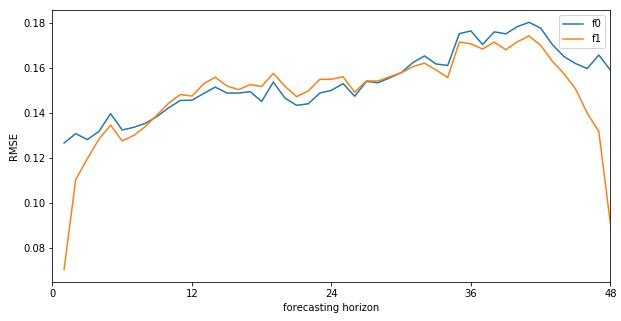
\includegraphics[width=0.8\columnwidth]{FIG/f0f1}
\caption{Error of predictor $f0$, $f1$ over horizons}
\label{fig:f0f1}
\end{figure}
The ensemble model is obtained by combining experts at different forecasting horizons. Based on the prediction performance on validation set, a hybrid model $f01$ is formed by choosing $f1$ at horizons close to the available data and $f0$ at other forecasting horizons.

\subsubsection{Simple Average}
The mean-squared-error (MSE) of an predictor $\hat{\theta}$ with respect to the real value $\theta$ is defined as
\begin{equation}
    MSE(\hat{\theta}) = E_{\hat{\theta}}[(\hat{\theta} - \theta)^2] = Var_{\hat{\theta}}(\hat{\theta}) + Bias_{\hat{\theta}}(\hat{\theta}, \theta)^2
\end{equation}
The first hybrid approach is aimed at reducing the bias by choosing the best model at different horizons. The variance can be simply reduced by averaging the predictions of multiple models. Table \ref{tab:RMSE} shows the averaged prediction has less error than the best single model in layer 2.

\subsubsection{Stacked Regression}
Suppose we have a set of predictors  $f_1(x), \cdots, f_K(x)$, instead of selecting a single one from the set, a more accurate predictor can be obtained by combining them. We restrict attention to linear combinations
\begin{equation}
    f(x) = \sum_{k=1}^K \alpha_k f_k(x)
\end{equation}
In the simple average approach, $\alpha_k = \frac{1}{K}$ is a constant. Given samples $\{(x_n,y_n),n=1,\cdots,N\}$, we learn the coefficient $\alpha_k$ to minimize $\sum_{n=1}^N (y_n - \sum_{k=1}^K \alpha_k f_k(x))^2$. Since the single model predictions are highly correlated, we use ridge regression with regularization term $\sum_k \alpha_k^2 = s$. %It was pointed out in \cite{Breiman1996} that for non-negative coefficients $\alpha_k$, the trained linear combination will be better than the best single model in set $\{f_1(x), \cdots, f_K(x)\}$. %The procedure of training stacked regression is as follows :
%\begin{enumerate}
%    \item Split the training set into two sets (train \& holdout)
%    \item Train multiple base models on the first set (train)
%    \item Test these base models on the second set (holdout)
%    \item Train a high-level meta-model. Use the predictions from step 3 (out-of-folds predictions) as inputs (feature), and the actual values (target) as outputs (see Figure \ref{fig:stack})
%\end{enumerate}
%
%\begin{figure}[h]
%\centering
%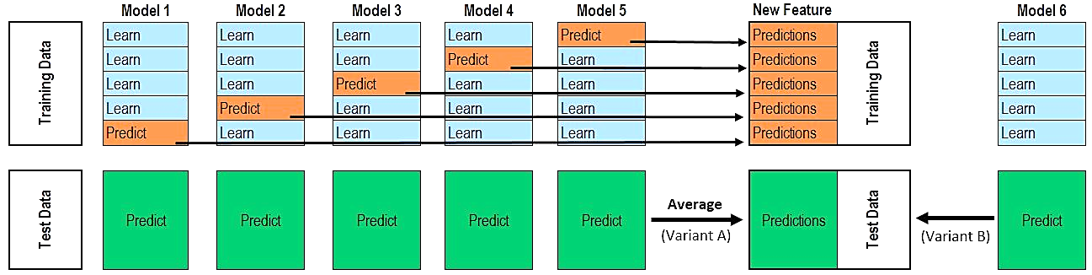
\includegraphics[width=0.9\columnwidth]{FIG/stack}
%\caption{Stacked Regressions}
%\label{fig:stack}
%\end{figure}



\section{Experiment Result}
The dataset comes from a Kaggle competition\footnote{https://www.kaggle.com/c/GEF2012-wind-forecasting}, in which hundreds of teams have submitted their prediction results. The performance of the proposed approach is compared with the winner's approach \cite{SILVA2014395} as well as two neural network models Node Decoupled Extended Kalman Filter trained Recurrent Neural Network (NDEKF\_RNN) \cite{Kanna13} and AWNN \cite{7894735}. The performance of the prediction models is evaluated by RMSE and MAE. Note that all power values were normalized to 0-1 range, which enables scale-free comparison on multiple farms.

In this work, we proposed a three-layer hybrid model for wind power prediction. Experiment results on the same public dataset show that our model has the best performance compared with several existing approaches (Table \ref{tab:RMSE}). It also shows the prediction error for single models in each layer and for the hybrid model. RMSE of the proposed hybrid model is 0.14508, which outperforms the state-of-the-art approach and the neural network models. The performance of persistence model and random guess are also listed for reference.

\begin{table}
\caption {Prediction Error in RMSE for Comparison.}
\begin{center}
\resizebox{\columnwidth}{!}{
\begin{tabular}{|c|c|c|}
\hline
model                   & note                      & RMSE              \\ \hline\hline
Linear Regression       & layer 1                   & 0.17390           \\ \hline
$f$0                    & layer 2                   & 0.15435           \\ \hline
$f$1                    & layer 2                   & 0.14997           \\ \hline
$f$6                    & layer 2                   & 0.15704           \\ \hline
$f$7                    & layer 2                   & 0.15777           \\ \hline
$f$10                   & layer 2                   & 0.15297           \\ \hline
$f$11                   & layer 2                   & 0.15390           \\ \hline
\textbf{$f$12}          & \textbf{layer 2}          & \bf{0.14914}      \\ \hline
$f$13                   & layer 2                   & 0.14949           \\ \hline
$f$15                   & layer 2                   & 0.15045           \\ \hline
$f$01                   & layer 3                   & 0.14873           \\ \hline
simple average          & layer 3                   & 0.14695           \\ \hline\hline
\textbf{Proposed}       & \textbf{layer 3}          & \bf{0.14508}      \\ \hline
Leustagos \cite{SILVA2014395}  & winner's approach         & 0.14567           \\ \hline
DuckTile \cite{HONG2014357}           & local linear regression   & 0.14719           \\ \hline
Duehee Lee \cite{HONG2014357}         & neural network \& Gaussian process & 0.15501  \\ \hline
AWNN \cite{7894735}     & wavelet neural network    & 0.15014           \\ \hline
NDEKF\_RNN \cite{Kanna13} & recurrent neural network  & 0.15347           \\ \hline
PERSIST                 & persistence model         & 0.35366           \\ \hline
Random                  & random guess              & 0.46070           \\ \hline
\end{tabular}
}
\label{tab:RMSE}
\end{center}
\vspace*{-5mm}
\end{table}

In this task, the WPP model predicts 48-hour ahead hourly wind power generation at 7 wind farms. Figure \ref{fig:horizon} plots the prediction error over 48 forecasting horizons, in which $f7$ and $f12$ are the worst and the best model in the second layer. Including historical observations significantly improves the performance at horizons close to the available data, that is, the first and last few hours. %Figure \ref{fig:error_farm} plots the prediction error over 7 wind farms. All models show larger error in farm 3 and 5, probably due to the inaccurate NWP forecasts.

\begin{figure}[b]
\centering
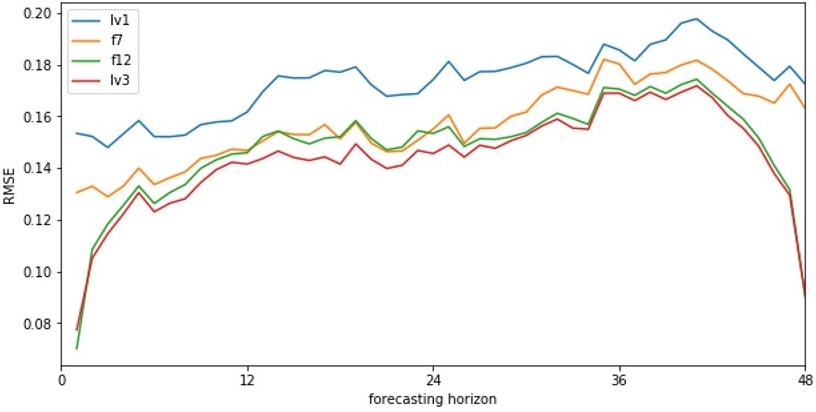
\includegraphics[width=0.8\columnwidth]{FIG/horizon}
\caption{Prediction error over forecasting horizons}
\label{fig:horizon}
\vspace*{-5mm}
\end{figure}

%\begin{figure}
%\centering
%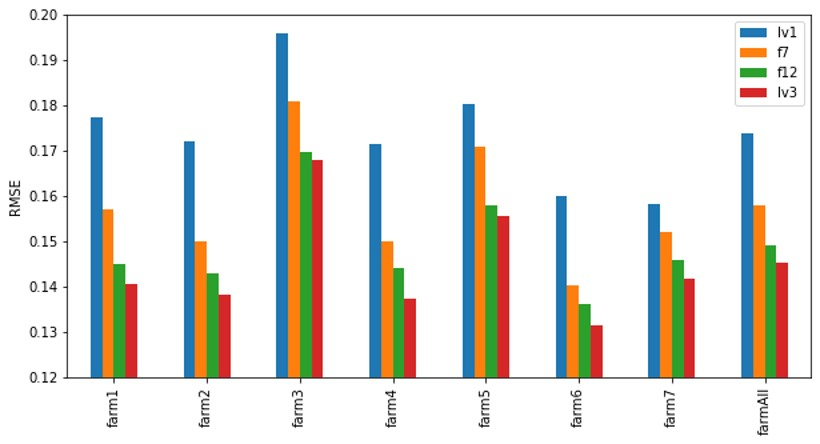
\includegraphics[width=0.8\columnwidth]{FIG/error_farm}
%\caption{Prediction error over wind farms}
%\label{fig:error_farm}
%\end{figure}

Model performance varies over forecasting horizons. %Figure \ref{fig:section} listed the performance over four horizon periods $[1,12]$, $[13,24]$, $[25,36]$ and $[37,48]$, in which the first row is the average over four periods.
A comparison over horizon period $[13, 36]$ with AWNN \cite{7894735} and NDEKF\_RNN \cite{Kanna13} is displayed in Table \ref{tab:section}. Note that the horizon period $[13,36]$ is where the neural network models have the largest improvement over the persistence baseline. Figure \ref{fig:actual} shows actual and predicted wind power on farm 2.

%\begin{figure}
%\centering
%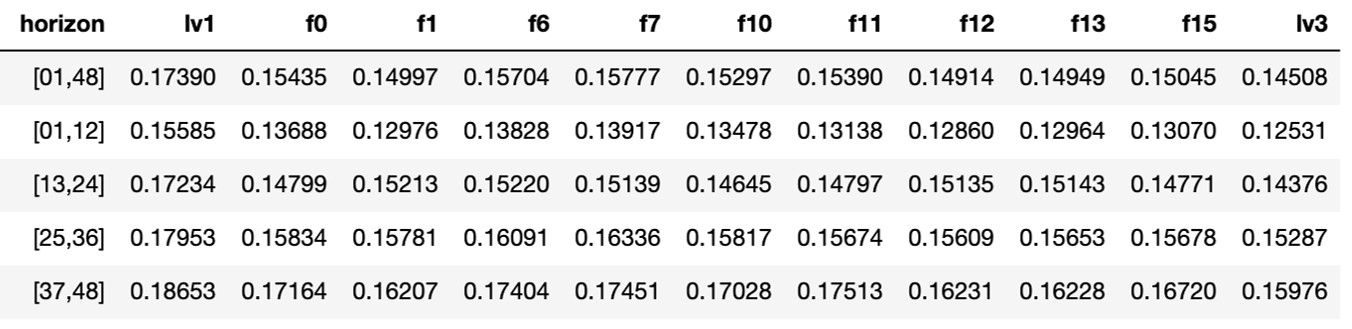
\includegraphics[width=0.9\columnwidth]{FIG/section}
%\caption{Prediction error over four horizon periods}
%\label{fig:section}
%\vspace*{-3mm}
%\end{figure}

\begin{table}[ht]
\caption {Prediction error over horizon period $[13,36]$}
\begin{center}
\resizebox{\columnwidth}{!}{
\begin{tabular}{|c|c|c|c|}
\hline
model                   & note                      & RMSE         & MAE            \\ \hline\hline
\textbf{Proposed}       & \textbf{layer 3}          & \bf{0.1496}  & \bf{0.1055}    \\ \hline
AWNN \cite{7894735}     & wavelet neural network    & 0.1531       & 0.1172         \\ \hline
NDEKF\_RNN \cite{Kanna13}& recurrent neural network & 0.1690       & 0.1280         \\ \hline
PERSIST                 & persistence model         & 0.3710       & 0.2725         \\ \hline
\end{tabular}
}
\label{tab:section}
\end{center}
\vspace*{-5mm}
\end{table}

\begin{figure}[t]
\centering
%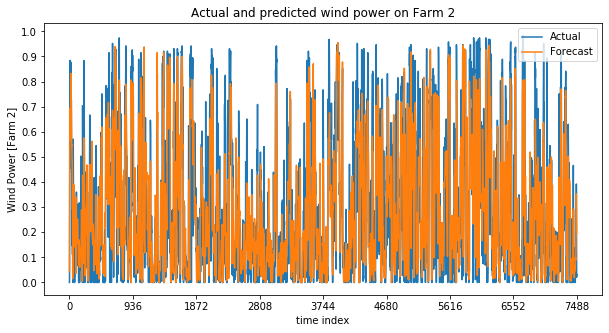
\includegraphics[width=0.9\columnwidth]{FIG/actual}
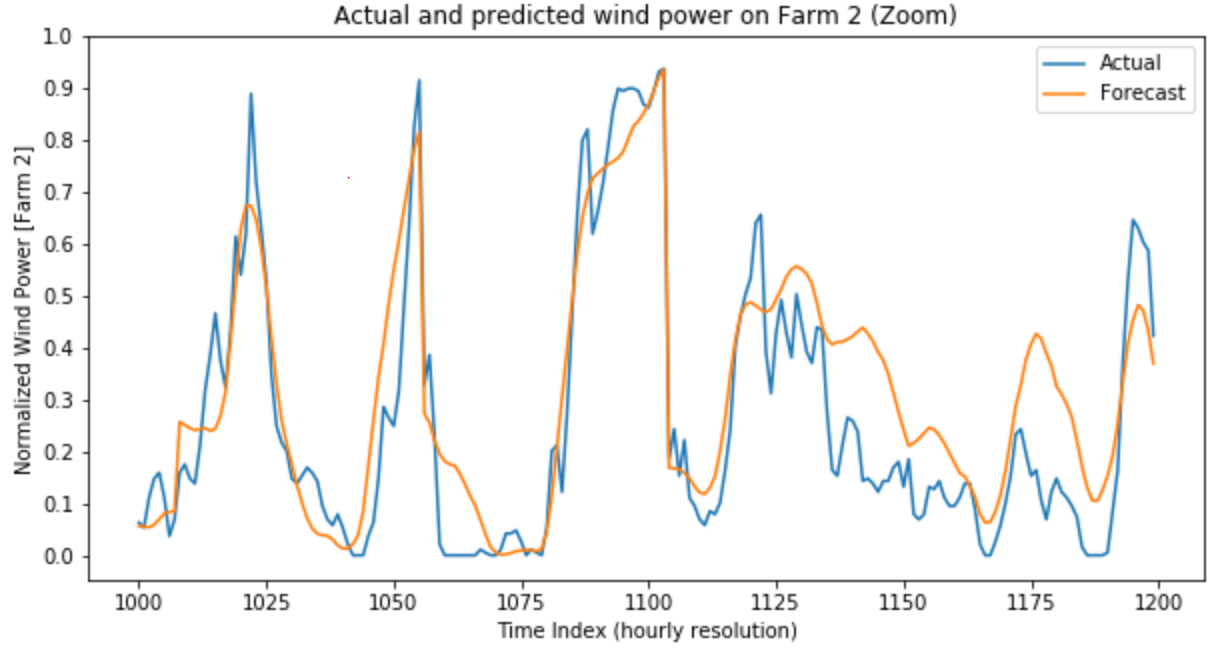
\includegraphics[width=0.85\columnwidth]{FIG/actualzoom}
\caption{Actual and Predicted Wind Power}
\label{fig:actual}
\vspace*{-3mm}
\end{figure}



\section{Conclusion}
This paper proposed a three-layer hybrid model for wind power prediction. The useful information comes from two aspects: the NWP wind forecast and the historical wind power measurement. We developed multiple models targeting at different aspects of knowledge. The hybrid model integrates the physical and statistical models specialized for short and long forecasting horizons. Experiment results on a public competition dataset show that the proposed prediction model has the best performance compared with the state-of-the-art approach as well as several neural network models.
%Hybrid approach offers significant improvement over the single models. It combines different characteristics in the single models and reduces the bias and variance of the prediction result. The best individual model $f12$ is trained on 7 farms and 48 horizons separately, and takes into account the historical observations. The smoothing trick alleviates the effect of outliers by considering the correlation over time and location. It is found that recurrent neural network models including adaptive wavelet, extended Kalman filter and LSTM do not show advantage on this dataset. The use of recursive feature improves the prediction only on short forecast horizons.
Future work is to incorporate discrete wavelet transform with LSTM network for short-term forecasting. Another direction is to develop power prediction models for solar energy and produce probabilistic predictions.




% An example of a floating figure using the graphicx package.
% Note that \label must occur AFTER (or within) \caption.
% For figures, \caption should occur after the \includegraphics.
% Note that IEEEtran v1.7 and later has special internal code that
% is designed to preserve the operation of \label within \caption
% even when the captionsoff option is in effect. However, because
% of issues like this, it may be the safest practice to put all your
% \label just after \caption rather than within \caption{}.
%
% Reminder: the "draftcls" or "draftclsnofoot", not "draft", class
% option should be used if it is desired that the figures are to be
% displayed while in draft mode.
%
%\begin{figure}[!t]
%\centering
%\includegraphics[width=2.5in]{myfigure}
% where an .eps filename suffix will be assumed under latex,
% and a .pdf suffix will be assumed for pdflatex; or what has been declared
% via \DeclareGraphicsExtensions.
%\caption{Simulation results for the network.}
%\label{fig_sim}
%\end{figure}

% Note that the IEEE typically puts floats only at the top, even when this
% results in a large percentage of a column being occupied by floats.


% An example of a double column floating figure using two subfigures.
% (The subfig.sty package must be loaded for this to work.)
% The subfigure \label commands are set within each subfloat command,
% and the \label for the overall figure must come after \caption.
% \hfil is used as a separator to get equal spacing.
% Watch out that the combined width of all the subfigures on a
% line do not exceed the text width or a line break will occur.
%
%\begin{figure*}[!t]
%\centering
%\subfloat[Case I]{\includegraphics[width=2.5in]{box}%
%\label{fig_first_case}}
%\hfil
%\subfloat[Case II]{\includegraphics[width=2.5in]{box}%
%\label{fig_second_case}}
%\caption{Simulation results for the network.}
%\label{fig_sim}
%\end{figure*}
%
% Note that often IEEE papers with subfigures do not employ subfigure
% captions (using the optional argument to \subfloat[]), but instead will
% reference/describe all of them (a), (b), etc., within the main caption.
% Be aware that for subfig.sty to generate the (a), (b), etc., subfigure
% labels, the optional argument to \subfloat must be present. If a
% subcaption is not desired, just leave its contents blank,
% e.g., \subfloat[].


% An example of a floating table. Note that, for IEEE style tables, the
% \caption command should come BEFORE the table and, given that table
% captions serve much like titles, are usually capitalized except for words
% such as a, an, and, as, at, but, by, for, in, nor, of, on, or, the, to
% and up, which are usually not capitalized unless they are the first or
% last word of the caption. Table text will default to \footnotesize as
% the IEEE normally uses this smaller font for tables.
% The \label must come after \caption as always.
%
%\begin{table}[!t]
%% increase table row spacing, adjust to taste
%\renewcommand{\arraystretch}{1.3}
% if using array.sty, it might be a good idea to tweak the value of
% \extrarowheight as needed to properly center the text within the cells
%\caption{An Example of a Table}
%\label{table_example}
%\centering
%% Some packages, such as MDW tools, offer better commands for making tables
%% than the plain LaTeX2e tabular which is used here.
%\begin{tabular}{|c||c|}
%\hline
%One & Two\\
%\hline
%Three & Four\\
%\hline
%\end{tabular}
%\end{table}


% Note that the IEEE does not put floats in the very first column
% - or typically anywhere on the first page for that matter. Also,
% in-text middle ("here") positioning is typically not used, but it
% is allowed and encouraged for Computer Society conferences (but
% not Computer Society journals). Most IEEE journals/conferences use
% top floats exclusively.
% Note that, LaTeX2e, unlike IEEE journals/conferences, places
% footnotes above bottom floats. This can be corrected via the
% \fnbelowfloat command of the stfloats package.








% conference papers do not normally have an appendix


% use section* for acknowledgment
%\section*{Acknowledgment}
%The authors would like to thank Pierre Huyn, Kishan Guddanti, and Zehan Xu for their comments and suggestions.

%\clearpage




% trigger a \newpage just before the given reference
% number - used to balance the columns on the last page
% adjust value as needed - may need to be readjusted if
% the document is modified later
%\IEEEtriggeratref{8}
% The "triggered" command can be changed if desired:
%\IEEEtriggercmd{\enlargethispage{-5in}}

% references section

% can use a bibliography generated by BibTeX as a .bbl file
% BibTeX documentation can be easily obtained at:
% http://mirror.ctan.org/biblio/bibtex/contrib/doc/
% The IEEEtran BibTeX style support page is at:
% http://www.michaelshell.org/tex/ieeetran/bibtex/
\bibliographystyle{IEEEtran}
\bibliography{mybib}
% argument is your BibTeX string definitions and bibliography database(s)
%\bibliography{IEEEabrv,../bib/paper}
%
% <OR> manually copy in the resultant .bbl file
% set second argument of \begin to the number of references
% (used to reserve space for the reference number labels box)
%\begin{thebibliography}{1}

%\bibitem{IEEEhowto:kopka}
%H.~Kopka and P.~W. Daly, \emph{A Guide to \LaTeX}, 3rd~ed.\hskip 1em plus
%  0.5em minus 0.4em\relax Harlow, England: Addison-Wesley, 1999.

%\end{thebibliography}


% that's all folks
\end{document}


% [1]. Long-Term Wind Speed Forecasting and General Pattern Recognition Using Neural Networks
% [2]. A Review of Wind Power Forecasting Models
% [3]. A Comparative Study on the Impact of Grid Code Regulations on Stability of Wind Integrated Power Systems
% [4]. Review of international grid codes for wind power integration: Diversity, technology and a case for global standard
% [5]. Mid-to-long term wind and photovoltaic power generation prediction based on copula function and long short term memory network
% [6]. Different Models for Forecasting Wind Power Generation: Case Study
% [7]. A Case-Study of Wind Turbine Power Forecasting Using Machine Learning Techniques
% [8]. S. Fan, J. Liao, R. Yokoyama, L. Chen, and W.-J. Lee, “Forecasting the Wind Generation Using a Two-Stage Network Based on Meteorological Information,” IEEE Trans. Energy Convers., vol. 24, no. 2, pp. 474–482, june 2009.
% [9]. Long Term Wind Power Forecast Using Adaptive Wavelet Neural Network
% [10]. Wind Power Short-Term Prediction Based on LSTM and Discrete Wavelet Transform
% [11]. Global Energy Forecasting Competition 2012
% [12]. Wang, C.; Zhang, H.; Fan, W.; Ma, P. A new chaotic time series hybrid prediction method of wind power based on EEMD-SE and full-parameters continued fraction. Energy 2017, 138, 977–990
% [13]. Chang, W.-Y. A literature review of wind forecasting methods. J. Power Energy Eng. 2014, 2, 161–168.
% [14]. Wang, D.; Lou, H.; Grunder, O.; Lin, Y. Multi-step ahead wind speed forecasting using an improved wavelet neural network combining variational mode decomposition and phase space reconstruction. Renew. Energy 2017, 113, 1345–1358.
% [15] L. Lazic, G. Pejanovic, and M. Zivkovic, “Wind forecasts for wind power generation using the Eta model,” Renewable Energy, vol. 35, no. 6, pp. 1236-1243, June 2010
% [16] J. Tambke, et al., “Short-term Forecasting of Offshore Wind Farms Production – Developments of the Anemos Project”. In Proc. of the European Wind Energy Conference 2006, Athens, Greece, 27/2-2/3 2006.
% [17]. Patel, M.R. Wind and Solar Power Systems: Design, Analysis, and Operation; CRC Press: Boca Raton, FL, USA, 2005.
% [18]. A Feature Engineering Approach
% [19]. XGBoost: A Scalable Tree Boosting System
% [20]. Stacked regressions
% [21]. Improved RNN and AWNN based Wind Power Forecast using Meteorological Inputs
